\chapter{Literature Review}

\section{Cooperativism and Co-ops}

\paragraph{} In order to define cooperativism, it may be best to start with what it is not. Cooperatives as a structure are not the same as the act of collaborating. In order for a collaboration to be cooperative in nature, that collaboration would need take place within a group that is democratically-run, typically practiced as one-member-one-vote, with the members collectively deciding how their resources will be used to benefit them \autocite[54]{ratner_cooperativism_2009}. In the case of game development, teams of developers can collaborate in order to produce a game but that collaboration would not be cooperative unless its results were jointed owned and managed collectively by all the members. As such, cooperativism can best be described as the organizational principle in which the results of a group's collaboration are jointly-owned and democratically-controlled by its members.

\paragraph{} Co-ops are enterprises that are organized to practice cooperativism. These types of institutions are owned by the people who work there who then manage it democratically. This structure allows them to be run for member-benefit as each member of the co-op has the ability to directly participate in the decision-making process. The International Cooperative Alliance has adopted seven principles, based on the Rochdale Principles, by which cooperatives are to put the value of cooperativism to practice: voluntary and open membership, democratic member control, member economic participation, autonomy and independence; education, training and information; cooperation among cooperatives, and concern for community \nocite{international_cooperative_alliance_cooperative_nodate}.

\paragraph{}

\begin{figure}[h!]
    \centering
    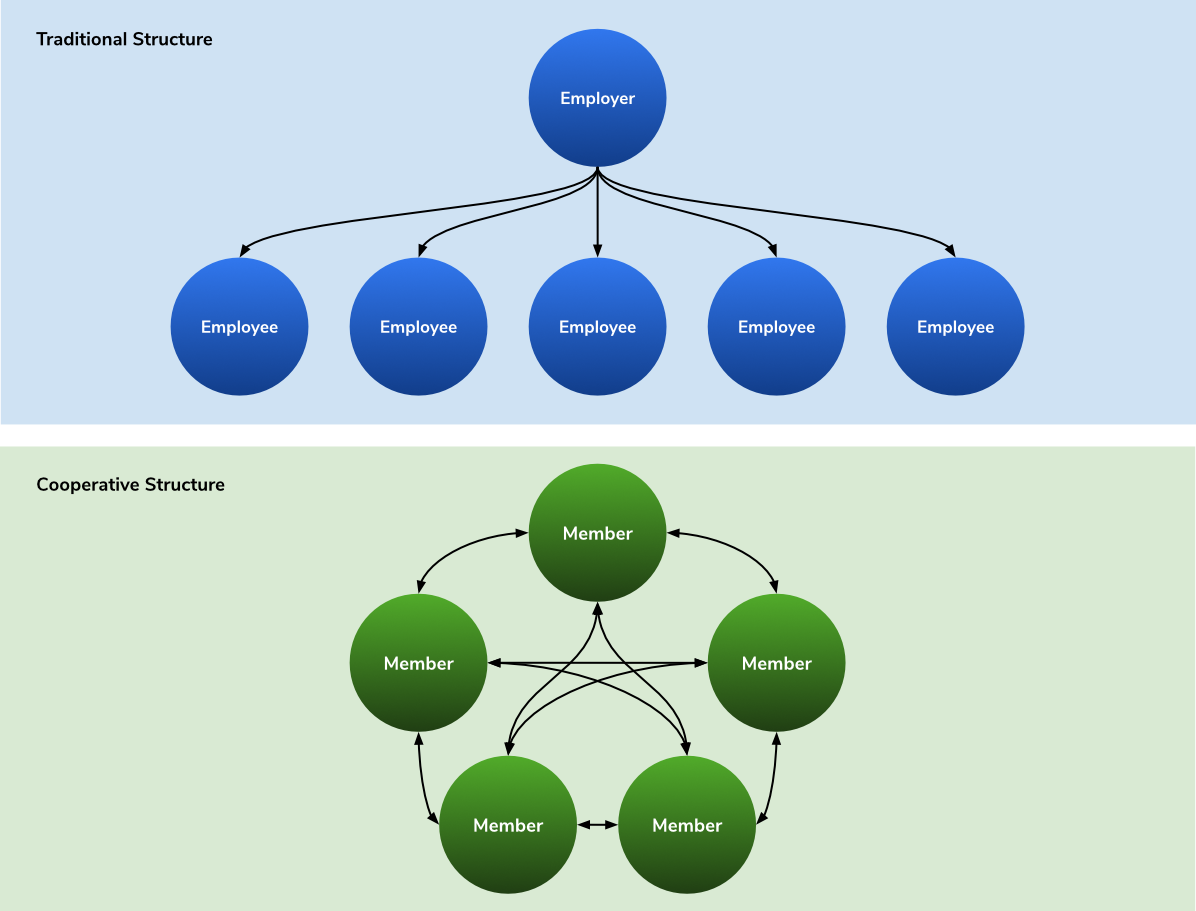
\includegraphics[width=\linewidth]{Figures/StructureComparison.png}
    \caption{A comparison between traditional and cooperative enterprise structures.}
\end{figure}

\paragraph{Voluntary and Open Membership} Cooperative teams are open to all persons interested and willing to accept the responsibilities of membership. Members of cooperatives voluntarily give their skills and resources to the team in order to contribute to a mutual goal. Membership of cooperative teams is available to all without gender, racial, political, religious or social discrimination. Fraternal benefit societies are an exception to this as their membership often shares one of the previously mentioned characteristics \autocite[16]{boland_introduction_2017}.

\paragraph{Democratic Member Control} This refers to both the practice of management through one-member-one-vote and the collective ownership of the results of the teamwork. Decisions within these types of teams require a consensus since each member has a vote; the validation for choices made comes from the majority of the voting team members to affirm them. The methods by which cooperative teams institute these paradigms vary based on their size, resources, and needs. Larger cooperative teams, for example, may elect their own management to manage any complexities or delegate some decision-making \autocite[21]{northcountry_cooperative_foundation_worker_2006}. 

\paragraph{Member Economic Participation} Since cooperatives are collectively-owned, each member contributes equitably and democratically controls their co-op's capital. Members of co-ops often receive financial benefits such as payment for their contributions. They also control how the capital is spent. Common uses for capital at a co-op include development, building reserves, and support for external activities. Co-ops being operated for member benefit should not be misconstrued to mean they should not seek a profit; the distribution of the profit is part of the participation benefits \autocite[29]{boland_introduction_2017}. 

\paragraph{Autonomy and Independence} Co-ops are self-organized and controlled by their members; their decisions are the decisions of the co-op. When a co-op enters agreements, raises revenue from external sources, or engages in other external relations, they do so on their own accord and at the membership's consent. Relations with external groups should also help to maintain the autonomy of the co-op. 

\paragraph{Education, Training and Information} For member of a co-op to effectively contribute, they need to know how to do so and how to operate within a cooperative team. Additionally, co-ops also educate the general public about the benefits of cooperativism.

\paragraph{Cooperation Among Cooperatives} To strengthen the cooperative community, co-ops seek to collaborate. By sharing resources and working together on projects, co-ops can build support networks that benefit all their members. This also includes forming federations of co-ops to facilitate this collaboration.

\paragraph{Concern for Community} Co-ops work within their communities to engage in and promote sustainable policy. As with the other principles, community engagement is at the discretion of the membership. 

\paragraph{} Cooperative enterprises come in varying forms and serve varying purposes. Co-ops can be focused on a need within their community such as childcare or housing, an industry such as the arts or agriculture, or provide more general services such as utilities or financial assistance. What distinguishes them from conventional firms is their ownership and management by their members. Cooperatives also often form federations in order to cooperate amongst one another and share resources \autocite{boland_introduction_2017}. 

\paragraph{} This study focuses on teams as they would exist in a worker-owned cooperative. These are co-ops in which workers combine their skills and resources in order to gain steady employment and income. This study focuses on this type of co-op because game studios that are cooperatively owned would be considered worker co-ops. Teams of developers in these types of studios use their skills, such as design, art, or programming, in order to create employment and income for themselves by producing games in a democratic workspace. Like conventional game studios, they can either produce and sell their own games or offer development as a service.

\paragraph{} The literature consensus is that both cooperativism and co-ops are predicated on collective ownership and some form of democratic decision-making. Carl Ratner does not offer any explicit strategies for implementing these values in \textit{Cooperativism: A Social, Economic, and Political Alternative to Capitalism} but rather describes the characteristics of various stages of cooperative activity (54-60). By contrast, the Northcountry Cooperative Foundation's \textit{Worker Co-op Toolbox} and Michael Boland's \textit{An Introduction to Cooperation and Mutualism} discuss strategies for successfully starting a co-op, structuring co-ops and handling elected management. Both of the aforementioned texts refer to the International Cooperative Alliance's seven cooperative principles.

\section{Historical Overview}

\paragraph{} Worker-owned cooperatives first came to public attention as part of the labor movement during the Industrial Revolution in Europe and the United States. The transitioning of the production towards manufacturing processes during this time led to a decline in various job sectors. This resulted in large sections of the workforce transitioning to wage labor which could be insecure especially during economic downturns. In response to these changes, workers started to organize their businesses and manage them democratically \autocite{adams_putting_1992}. In 1844, the Rochdale Society of Equitable Pioneers established the Rochdale Principles which are the basis for the seven principles of the modern cooperative movement as defined by the International Cooperative Alliance \autocite{thompson_co-op_1994}.

\paragraph{} Co-ops continue to exist to this day and are part of the overall global economy. In 2018, five pilot co-ops were given a \$1 million grant by Google to support economic development of cooperatives in the digital economy through critical analysis and designing of open source tools \autocite{the_new_school_trebor_2018}. Roughly 12\% of the world population were cooperators at any of the roughly three million cooperatives worldwide in 2020 \autocite{world_cooperative_monitor_exploring_2020}. Examples of established co-ops today include the Mondragon Corporation in Spain, Suma Wholefoods in the United Kingdom, and Means LLC in the United States.

\paragraph{}

\begin{figure}[h!]
    \centering
    
\includegraphics[width=\linewidth]{Figures/GlobalCoopsGDP.png}
    \caption{The 300 co-ops worldwide with the highest GPD per capital in 2018 according to the World Cooperative Monitor.}
\end{figure}

\paragraph{} The longevity of the cooperative movement can be explained by the benefits their members receive; one of these is their resiliency. A study of three year survival rates of businesses in France from 2013 finding that worker co-ops had an 80\% to 90\% rate while the overall survival rate was 66\% \autocite{kruse_relative_2013}. A survival analysis of co-ops in Uruguay from 1999 to 2008 found that they had a roughly 29\% smaller chance of closing than traditional firms in similar industries \autocite{burdin_are_2014}. This may be explained as a possible outcome of running an enterprise for member benefit; planning for longevity benefits each member by providing them the economic security necessary to do their work.

\paragraph{} Worker co-ops can also benefit each member's productivity and emotional well-being. A 1995 study of co-ops in the timber industry in the United States found that they were 6\% - 14\% more efficient \autocite{craig_participation_1995}. Members of co-ops also report being happier with their job with a study of home health aides in the United States finding higher satisfaction rates among those who were members of a co-op \autocite{kruse_effects_2013}. Since members of co-ops are able to decide how their work takes place, they can facilitate working conditions that best fit their needs.

\paragraph{} Cooperatives in the game industry are organizations of developers that pool their skills and resources together to produce games. One type of game co-op operates similarly to the conventional studio in that they create games they can use to generate enough revenue. However, the co-op seeks to do so in order to foster an equitable and sustainable environment for members to develop games collaboratively by offering their human capital in the form of their work and in some cases financial capital. Steve Filby of Motion-Twin shared the following thoughts with Game Workers Unite about why they chose to form a co-op:

\begin{quote}
    \item{} The guys started off as a bunch of friends hanging out making games, so there was naturally no boss. When they started to make money from games and needed to pay taxes they realised they needed a legal structure/business entity, but the traditional company structure meant you were pretty much obligated to have a boss and that the equity and gain that could be made on company shares without participation was not at all what they wanted to do \autocite{game_workers_unite_worker_2021}.
\end{quote}

\paragraph{} The structure of a worker co-ops best suited the needs of Motion-Twin by allowing them to set up a company structure that reflected the egalitarian essence of their team. They could have a legally recognized business entity while also keeping control of their projects to those who are engaged in their production. On the topic of their decision-making process, Filby also added the following:

\begin{quote}
    \item{} Zero hierarchy, equal pay, equal say. There are two people who wear the "Co-CEO" hats who have the glorified role of signing for things, but all big decisions must be voted by the simple majority and unanimously if they're gong to change the rules that govern the co-op. Democracy is maintained through constant vigilance and ritual combat (also known as talking, A LOT). \autocite{game_workers_unite_worker_2021}.
\end{quote}

\paragraph{} Filby stresses the role of democratic decision-making at Motion-Twin by identifying that all major decisions are made through voting. He also notes the need for effective communication with the co-op to maintain this structure.

\paragraph{} Another example of this type of co-op is The Glory Society based out of the United States. Scott Benson, one of the members of The Glory Society, was asked by Game Workers Unite about the benefits of organizing a co-op studio and answered the following:

\begin{quote}
    \item{} \ldots We're all a lot more signed onto the project and personally invested because it belongs to all of us. Even if you're the coolest boss ever, you're still someone's boss, which means you're always wielding this power over someone even if you promise never to abuse it. Removing that does wonders for morale. I think we all work better creatively as well since we have to actually talk with one another in ways that if we were a top-down studio we wouldn't be as encouraged to do. And credit is naturally a bit more spread around, since it's such a group thing as opposed to some visionary person and their employees. Also it means our schedules aren't dictated from on high, and we can work around our lives if need be, vote for vacation time, etc. \ldots There's lots of little things you don't even think about at first but are big changes from what we're all used to from previous jobs \autocite{game_workers_unite_worker_2021}.
\end{quote}

\paragraph{} Benson's list of the benefits of working at a co-op aligns with those identified in the previously mentioned studies on the productivity and happiness of co-op members. The ability for members to decide how they will work and what their schedule will allow them to shape the production to fit their needs.

\paragraph{} Another type of game co-op is one in which developers offer their skills to clients to make games or components of them. A driving motivation behind their formation is to prevent the insecurity that can often come with contract work in the game industry. In a 2019 presentation at the Game Developers Conference, Ian Thomas of Talespinners, a game co-op in the United Kingdom that develops narratives for clients, described how one of the benefits of the co-op was the credibility that came with having a brand that encouraged more clients to work with them. Another benefit he discussed was the ability for the members to create a fund that could provide financial assistance to members when necessary \autocite{game_developers_conference_embracing_2019}. Thomas is quoted by Game Workers United on the topic of how participating in a co-op has influenced his values as stating that:

\begin{quote}
    \item{} I think the key for me has been the realisation that the freelance economy is so precarious, and that anything we can do to alleviate that - and act as a template for others, to help them alleviate it - is incredibly valuable. The co-op has strengthened that belief. \autocite{game_workers_unite_worker_2021}.
\end{quote}

The insecurity of contract work that each of the members would have taken on individually was prevented in the case of Talespinners by having the co-op there to offer work and support the members financially. The alleviation of the precariousness of freelance work is a reflection of the resiliency of co-ops as discussed previously.

\paragraph{} In addition to the two previous types of co-ops in the game industry, there are also incubators that either serve co-ops or offer cooperative workspaces. For example, Dutch Game Garden in the Netherlands offers incubation, matchmaking and economic development services to the Dutch games industry \autocite{dutch_game_garden_about_nodate}. Another example of this type of co-op is Games Plus in Australia which provides hubs for game developers and other technology-related start-ups to co-locate and share their knowledge and resources \autocite{game_plus_home_nodate}.

\paragraph{} This study focuses on the development of games as it would take place in a democratic and cooperative group of developers. This would exclude the type of cooperative development that would take place in a firm that relies on only completing parts of a game or only serve to share resources. Examples of game co-ops that the model would apply to are Motion-Twin and Studio Black Flag, both located in Bordeaux, France as well as Pixel Pushers Union 512 in the United States because they produce a complete game from start-to-finish on democratic teams for the purpose sustaining each member's ability to work on games. This model could also be applied at co-ops that work with clients to produce full games with teams of developers such as the TESA Collective in the United States.

\section{Social Problems in Game Development}

% Reframe first paragraph to just be about social problems in game development, not based on ethnography.
% Change all mentions to ethnography to discussions of social issues.
%  Make sure to explicitly connect how social problems can impact decision-making in coops.

\paragraph{} Studying game development from an ethnographic approach reveals that problems that arise in its routine practice are often social rather than technical or theoretical. Ethnographic methods of research provide a means of understanding the connections between practices and objects in relation to the lived experiences of those who act them out \autocite{apperley_game_2012}. In terms of game development, ethnographic studies examine developers, tools, and their interactions to better understand the realities of day-to-day operations \autocite{whitson_what_2020}. This study focuses on social problems in game development because developing games in cooperative teams is a social experience that impacts the connections between developers and their tools.

\paragraph{} One example of a problem that arises when using this approach to examine game development practices involves the circumvention of a tool's limitations by developers to accomplish their goals. The tools developers use to make games act as the boundary objects in which development is confined. As developers identify what they can achieve with their tools, the production becomes shaped around those possibilities; this results in interactions between the developer and the tool become a form of negotiation. Jennifer Whitson describes this as "voodoo software" where the personification of a tool appears to exert agency that developers accommodate. It is the diplomatic engagement between the developer and the tool that requires social problem-solving skills \autocite{whitson_voodoo_2018}.

\paragraph{} Another example is that developers may need to educate each other on work traditionally reserved for their role within a production to align the team on parts of the pipeline. These types of processes typically require cross-education to synchronize or integrate the production. An example of this would be cross-training a team on source control to synchronize and maintains versions of the project. This exposes the trainee developers to aspects of the pipeline they may not have been previously and the learning curve for each developer will vary. This knowledge sharing may require social skills to effectively teach those who may not share the same mental model \autocite{whitson_what_2020}.

\paragraph{} The success of the previously mentioned form of knowledge sharing is also dependent on the educating developers' abilities to communicate their knowledge of the subject. Tacit knowledge is built from practice; it is the accumulation of understanding through application. Explicit knowledge, by contrast, focuses on understanding what something is. These types of knowledge are not opposites but rather components of understanding through action which is not easily transferable from person-to-person because that action is where one's knowledge may be altered. The translation of that knowledge into information that can be understood and applied also requires a building of understanding through action and as such one's ability to educate effectively is dependent on that \autocite{orlikowski_knowing_2002}.

\paragraph{} The aforementioned social problems require "soft" skills to resolve; these skills, in conjunction with the material work, are necessary to organize people and tools into a final output. This organization is referred to as heterogeneous engineering. While these arrangements are made to facilitate the creation of an artifact, they can be unstable and may fail to achieve that. This is applied alongside social coordination to recruit and align people and narrow down the potential options to get the team to agree on the scope and shape of the artifact. Failure of social unification within a team can result in problematic approaches to cooperation including coercion, division, and silencing \autocite{law_technology_1987}. 

\paragraph{} When teams of developers create a game, they need to engage in heterogeneous engineering. The creation of digital spaces and interactivity can require a wide range of skills and require aligning the developers with those skills who may have differing interests. Designing a game involves applying production skills like storytelling, programming, and art with social skills such as analysis and calculation; these require synchronization amongst the team to maintain development. Additionally, the tools used for development act as a boundary object that impacts this calibration by framing the production possibilities around the team's ability to engage with them. Heterogenous engineering in game development aligns the developers and tools together to successfully complete a game \autocite{whitson_what_2020}.

\paragraph{} Professional game development postmortems offer a mixed amount of analysis on the social dynamics that existed during production. Companies may be reluctant to share stories of these types of issues because these documents also serve as public relations tools that act as a testimony to the company's practices. The fear that a company may expose proprietary secrets often results in postmortems containing few details about the production short of issues with scope and planning. More personalized accounts of game development in postmortems can also be conflated with gossip where it is perceived as being potentially damaging to one's career to be critical of other people. This emphasis on technical problems paints only part of a broader picture; the heterogeneous engineering that goes into development is often disregarded \autocite{odonnell_everyday_2009}.

\paragraph{} Game development within cooperative teams is also exposed to the aforementioned social problems and those unique to that structure.  Members of co-op teams must still negotiate with their technology, align each other on vital pipeline procedures and educate each other on production and workflow techniques. These all take place in conjunction with the facilitation of joint management. While defining production around the limitations of the interactions between developers and their tools is an important component of cooperative game development, problems of alignment are especially important because a lack of synchronization among members makes decision-making more difficult. Effective communication is a vital step in preventing these problems from arising \autocite{game_developers_conference_embracing_2019}.

\section{Analysis}

\paragraph{} This study focuses on the applying cooperativism to game development to create a viable model for cooperative teams. While the literature reviewed on cooperativism offered extended conversations on elected management structures in co-ops, such as boards of directors, this topic was not discussed in the review as they are primarily relevant to larger cooperatives and simulating these structures in the experiment would require additional research participants. As a result, the scope of this study is limited to a cooperative team with no elected management which is similar to the structure found at small game development co-ops like Motion-Twin and The Glory Society. This study examined social problems in game development because the practice of cooperation introduces problems resulting from interactions between developers and their tools.  

\paragraph{} Cooperativism and game development are social practices requiring participants to interact with one another and their tools to achieve their goals. The efficacy of cooperative ownership and management can depend upon the ability of members within a team to foster an environment for open communication and consensus building. Similarly, game development as heterogeneous engineering requires developers arrange themselves and their tools into a production that can create the intended output. Both of these factors are present in cooperative game development. A lack of heterogeneous engineering among developers can undermine the cohesion necessary to make jointly make decisions about its production.  

\paragraph{} The research opportunity for this study lies in developing a model that can facilitate heterogeneous engineering within cooperative game development teams. The model's focus is fostering an environment that can produce the social interactions necessary for joint decision-making and production within these types of groups. The approach to the research and development of this model focuses on social problems because the problems previously mentioned are those of the connections between the developers and their tools in relation to the experience of cooperative management.